\documentclass[../3Wworkreport.tex]{subfiles}
\doublespacing
\setcounter{chapter}{0}
\setcounter{section}{0}
\pagenumbering{arabic}

\begin{document}
\chapter{Introduction}
\label{chap:intro}

Quantum computing has made large strides in the last couple decades, and is emerging as a field of particular interest for mathematicians, physicists, computer scientists, and electrical engineers. From a theoretical standpoint, developing algorithms that take advantage of quantum phenomena and characterizing the differences between quantum and classical computational algorithms is necessary to determine precisely what resources are needed for quantum computers to be considerably more effective than current computers. The qubit (quantum bit) is a basis for much of the theoretical framework, and its two-state design is analogous to the classical 0-1 framework of classical computers. Working in dimensions higher than two (qubits are renamed qudits to emphasize the $d$-dimensional systems), can yield some results that are more intuitive than results strictly in two dimensions.\\

One area of study is communication complexity, and how entangled particles can help physically separated parties perform calculations. Given a problem, the communication complexity is the minimum amount of information exchanged between the two parties needed to solve the problem \cite{kushilevitz2006}. Looking at the information that must be exchanged has ties to cryptography, secure communication channels, and distributed computation.\\

Another relevant topic of interest is known as the stabilizer sub-theory. It involves certain quantum operators (also called gates, which are mathematically represented by unitary matrices) and how quantum algorithms associated with these operators can be simulated efficiently on classical computers. Closely related to the formalism of stabilizers is the discrete Wigner function, which serves as both an intuitive approach to quantum states, and a mathematical representation of them. While both of these areas are quite technical, the reader should refer to \autoref{app:stabilizer} and \autoref{app:dwf} to get a better understanding of these topics.\\

While communication complexity and the stabilizer sub-theory are not typically overlapping topics of study, some problems coming from a communication complexity framework can be solved effectively by developing algorithms that are based upon the stabilizer formalism; one such problem is known as Raz's problem.\\

Raz's problem \cite{Raz1999} comes in two variants, but both are based off of the same premise. The following definitions are consistent across both variants: the two parties of interest are named Alice and Bob; $x \in \mathbb{R}^d$ is a unit vector, where $d$ is an odd prime number; $M_0$ and $M_1$ are orthogonal subspaces of $\mathbb{R}^d$; and $\vartheta \in \mathbb{R}$ where $0 \le \vartheta < 1/\sqrt{2}$.
\begin{prob}
Let Alice have the vector $x$, Bob have the subspaces $M_0$ and $M_1$, and both Alice and Bob have the value $\vartheta$. Alice and Bob must communicate to output the value 0 if the distance d($x,M_0) < \vartheta$, and 1 otherwise.
\end{prob}

\begin{prob}
Let Alice have $x$ and the subspaces $M_0, M_1$, Bob have an orthogonal matrix $U$, and both Alice and Bob have the value $\vartheta$. Alice and Bob must communicate to output the value 0 if the distance d($Ux,M_0) < \vartheta$, and 1 otherwise.
\end{prob}

The goal is to provide solutions to these problems that minimize the communication complexity between Alice and Bob. A visual representation of these problems can be seen in \autoref{fig:razproblem}. Raz showed that there exists a protocol that solves Problem 2 where the lower bound for its complexity, using probabilistic classical computation, is $\Omega(\sqrt{d})$, and its upper bound is $O(d^{3/4})$. There is also a bound for Problem 1 of $O(\sqrt{d})$. As stated by Raz, and further discussed by Buhrman et al., efficient quantum computational protocols, however, have a communication complexity of $\Theta(log\,d)$, demonstrating an exponential separation in complexity between the two methods \cite{Buhrman2009}. The purpose of this report is to develop a classical protocol that approaches these lower bounds in general, and in special cases behaves like the quantum protocols. In addition, characterizing the special cases and how the protocol behaves in general will be discussed.

\begin{figure}[!h]
\begin{center}
\subfloat[Raz's Problem 1]{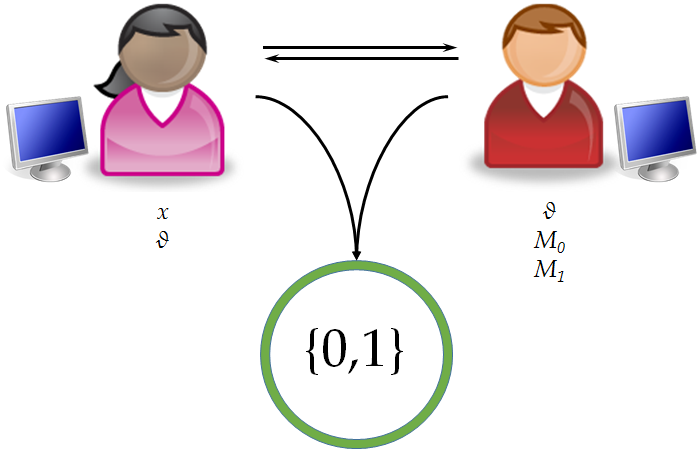
\includegraphics[width=0.5\textwidth]{Raz_prob1.png}}
\subfloat[Raz's Problem 2]{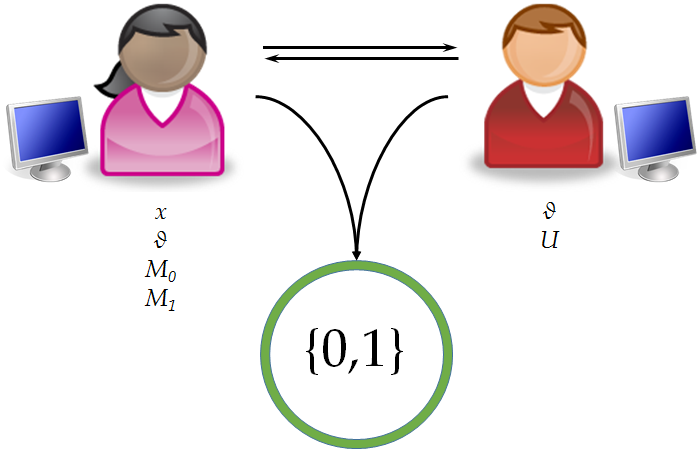
\includegraphics[width=0.5\textwidth]{Raz_prob2.png}}
\end{center}
\caption{Visualization of Raz's problems}
\label{fig:razproblem}
\end{figure}

\end{document}